\documentclass{article}
\usepackage{natbib}
\usepackage{graphicx}
\usepackage{amsmath}%American Ma th Society symbols
\usepackage[latin1]{inputenc}
\usepackage{mathrsfs}
\usepackage{amssymb}
\usepackage{graphicx}%Adding images, tables, and graphs
\usepackage{setspace}
\usepackage{epstopdf}
\usepackage[margin=1.5cm]{geometry}
\usepackage{cancel}
\usepackage{hyperref}
\usepackage{fullpage}
\usepackage{color}
\usepackage{threeparttable}
\usepackage{float}
\usepackage{breqn}
\usepackage{hyphenat}
\usepackage{mathtools}
\usepackage{textcomp}
\usepackage{authblk}
\usepackage{lscape}
\usepackage{dirtytalk}
\usepackage{appendix}


\hyphenation{matematica recuperar}
\setlength\parindent{24pt}

\pagenumbering{arabic}
\author[1]{Cassandra Duchan Saucedo\thanks{Federal Reserve Board of Governors, cassandra.r.duchan@frb.gov}}

\title{Bias-Motivated Incidents and Racial \& Ethnic Attrition: Relating Racial Hate Crimes to Americans' Reported Identities}
\date{DRAFT}

\begin{document}
\doublespacing
\maketitle

\section*{Abstract}

    Racial self-identity is malleable, with individuals choosing when, where, and whether to signal affiliation with particular groups. Accordingly, exogenous factors shaping the costs of a certain identity affect how one chooses to identify. One plausible determinant of racial identity is differential risk: individuals may be less likely to signal racial identities at higher risk. Specifically, crime that is inflicted \emph{because} of a person's identity --- hate crimes --- may motivate a person to affiliate differently. Because racial hate crimes are rare, they indicate strong racial tension and can serve as proxies for an area's discrimination against targeted groups. 
    
    This paper measures whether hate crimes in an area affect targeted groups' reported identities within the same area. I use the American Community Survey (ACS) and the Uniform Crime Report (UCR) for the United States from 2005 to 2016. I use a difference-in-differences design to test whether people reporting a particular ancestry or national origin (e.g., Nigerian or Mexican) are less likely to report the corresponding racial or ethnic identity (e.g., Black or Hispanic, respectively) following an increase in racially-motivated crime in their county. This approach follows findings that ancestry and origin reporting is more stable than racial and ethnic reporting (see Antman et al 2015). I find that people with Black ancestry are consistently less likely to identify as such in the presence of anti-Black hate crimes. People with Hispanic ancestry are generally more likely to identify as Hispanic in the presence of anti-Hispanic hate crimes.  
    
    \textbf{JEL Codes:} J1, D63, K42

\newpage


\section{Introduction}

    Today in the US, such crime is termed a hate crime: crime perpetrated against a person ``because of the other person's race, color, religion or national origin'' (Title 18 U.S.C. \§ 245). A greater salience of hate crimes committed against members of a particular racial identity may cause others change how they report their racial identity. Because racial crime is rare, it is indicative of greater racial tensions in an area and it can serve as a proxy for greater discrimination against targeted groups, overall. I find that people with Black ancestry are less likely to identify as such in the presence of anti-Black hate crimes in their geographic areas. 
    
    This paper builds on the literature investigating how changing incentives to identify with particular racial groups shape observed identifications. Antman et al (2015) use changes to affirmative action policies to show that reducing economic incentives to self-identity with a racial group causes individuals' associations with said group to decline. While increases in bias-motivated crime are not necessarily economic in nature, they can serve as a proxy for racial discrimination that does affect economic outcomes. Just as this decrease in economic incentives affected racial identifications, there may be a similar result with a decrease in other incentives to identify with a particular group.
    
    This paper demonstrates that race-based crime can alter the apparent demographics of a geographic area even without a change in population. Because American Community Survey (ACS) and Uniform Crime Report (UCR) data are both influential in civil rights policy work, policymakers should understand how they can interact. For instance, if there are apparently more hate crimes against a certain group while that group appears to be simultaneously decreasing, that could be due to changes in how individuals identify, rather than a change in the actual population living in the geographic area.
    
    The paper proceeds as follows: I tie incentives in self-identity to common sociological theories about experiences with crime and racial identity. From there, I examine the data, describing patterns in the racial, ethnic, and ancestry response in the ACS and providing detail on the UCR. The methodology divides identity groups and hate crimes into a few subcategories, and maps these categories to ancestry. These groups are Black and Hispanic people in particular, and the hate crimes committed specifically against these narrow groups.

\section{Data}

    The data used are from the 2005-2016 American Community Survey (ACS) and FBI Uniform Crime Report (UCR). UCR data are aggregated by local police jurisdictions and compiled by the FBI to create a comprehensive database of all reported hate crimes in the US. The hate crime data were connected to the ACS data through state, county, and, depending on the specification, year. 
    
    Individual ACS respondents to the ACS provide their self-reported racial and ethnic identities, and that of others living in their households. The list of racial options on the ACS includes categories such as \say{Black, African American or Negro}, \say{Asian Indian}, and \say{White}. Separately, ethnicity is divided into the categories of \say{No, not of Hispanic, Latino, or Spanish Origin} and different subsets of \say{Hispanic, Latino, or Spanish Origin} such as Puerto Rican. Race and ethnicity are listed as being separate entities that are not mutually exclusive. In this study, each group is treated separately to avoid multiple categorization. 
    
        % General Black Identification
		\begin{table}[!htbp] \centering 
          \caption{Self-Identified as Hispanic by Hispanic Ancestry} 
        \begin{tabular}{@{\extracolsep{5pt}} cccc} 
        \\[-1.8ex]\hline 
        \hline \\[-1.8ex] 
        Hispanic Ancestry Only & Hispanic \& Other Ancestry & No Hispanic Ancestry & Observations \\ 
        \hline \\[-1.8ex] 
        97.6\% & 74.4\% & 3.3\% & 2,858,387 \\ 
        \hline \\[-1.8ex] 
        Sample size & 15,024,310 & & \\
        \end{tabular} 
        \label{tab:id_anc_blk}
        \end{table} 
        
        % General Hispanic Identification
		\begin{table}[!htbp] \centering 
          \caption{Self-Identified as Black by Black Ancestry}
        \begin{tabular}{@{\extracolsep{5pt}} cccc} 
        \\[-1.8ex]\hline 
        \hline \\[-1.8ex] 
        Black Ancestry Only & Black \& Other Ancestry & No Black Ancestry & Observations \\ 
        \hline \\[-1.8ex] 
        96.0\% & 85.2\% & 0.44\% & 1,795,079 \\ 
        \hline \\[-1.8ex] 
        Sample size & 15,024,310 & & \\
        \end{tabular} 
        \label{tab:id_anc_hsp}
        \end{table} 
        %       & \\ 
        % \hline \\[-1.8ex] 
        
    In addition to racial and ethnic identification, ACS respondents can also report up to two ancestral responses. Ancestral options can describe an individual’s countries of origin or can  be tantamount to a racial identity. Figure \ref{fig:acs_anc} shows the portion on the ACS where respondents can provide their ancestral identities. Each ancestral response was mapped to a corresponding racial identification group based on its majority population. Individuals who did not provide any ancestral responses and individuals who provided any United States origin were removed from the dataset. Individuals with ancestral backgrounds are highly correlated with the associated racial and ethnic identities. Over 95 percent of those with exclusively Black and exclusively Hispanic ancestry identify with the associated groups (Tables \ref{tab:id_anc_blk} \& \ref{tab:id_anc_hsp}). There is more variation with those who have Black or Hispanic ancestry in combination with another ancestral grouping.
    
    Several restrictions were imposed on the sample to avoid confounding results. All individuals in the filtered data have to have resided in the same county over the past year to understand with greater certainty that they could have at least been aware of certain crime within their given geographic area during a given year. Furthermore, they must have provided at least one ancestral response, and cannot have responded to the ancestral question with the United States or any US state because such responses were not traceable to a specific racial or ethnic group. 
       
    \begin{figure}[h]
        \caption{ACS Ancestry Response}
        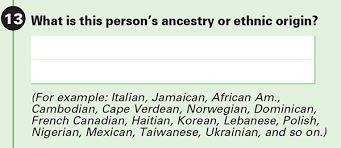
\includegraphics[scale = .75]{acs_ancestry.png}
        \label{fig:acs_anc}
        \centering
    \end{figure}
    
    From 2005 through 2016, 79,826 hate crimes were reported to the FBI (Uniform Crime Report 2005- 2016). Figure \ref{fig:hc} shows the breakdown of hate crimes during this time period, over 60 percent of which were racially or ethnically motivated. Anti-Black crimes account for the majority---54 percent---of racially and ethnically motivated hate crimes. Anti-Hispanic hate crimes account for 11 percent. Relative to their portions of the population, these racial or ethnic groups are the most disproportionately affected by targeted hate crime.  
    
    \begin{figure}[h]
        \caption{Hate Crime Distribution 2005-2016}
        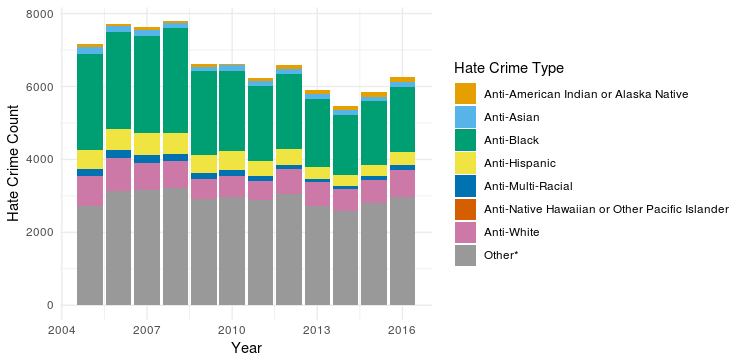
\includegraphics[scale = .7]{hc_dist_year.png}
        \label{fig:hc}
        \centering
    \end{figure}
    
    Figure \ref{fig:hc_map} shows that racially-motivated hate crimes are more frequent within populous, relatively diverse counties. Hate crimes per 1000 show a different story, with hate a higher number of hate crimes per 1000 occurring in smaller counties in the middle of the US (Figure \ref{fig:hc_cap_map}). This points to the importance of measuring identity relative to the local population size to understand the differential impact. For instance, Los Angeles County experienced over 2,800 racially-motivated hate crimes over the 11-year period but also is the largest county in the US; hate crimes per capita were around 0 for this county. Hate crimes per capita were highest in San Juan County, Colorado, with a population of less than 700 people. In these extreme cases, the differential impact seems clear. While most other counties fall somewhere between these cases---if a hate crime occurred within the county in this 11-year period---they are tangible examples. 
    
    \begin{figure}[h]
        \centering
        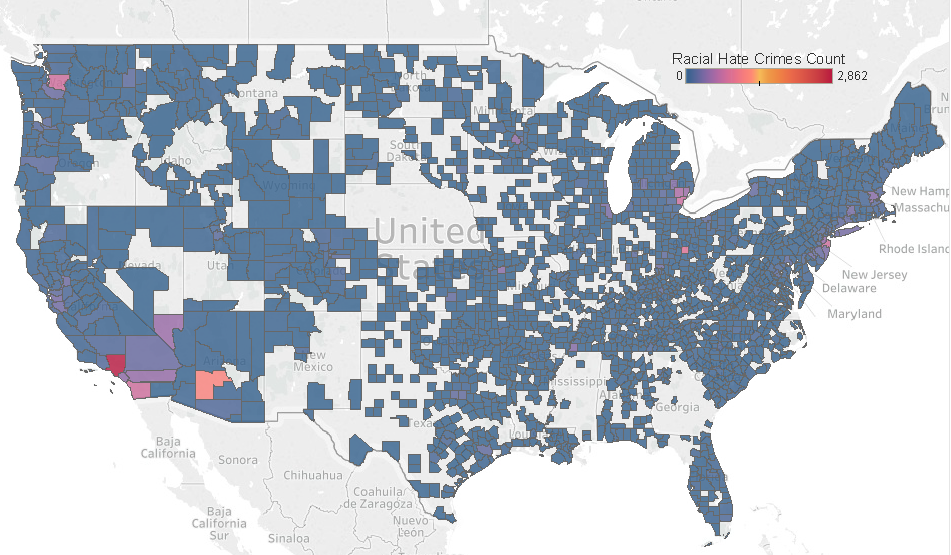
\includegraphics[scale = .6]{all_hc_2005_2016.png}
        \caption{US Mainland Hate Crime Distribution 2005-2016}
        \label{fig:hc_map}
    \end{figure}

    \begin{figure}[h]
        \centering
        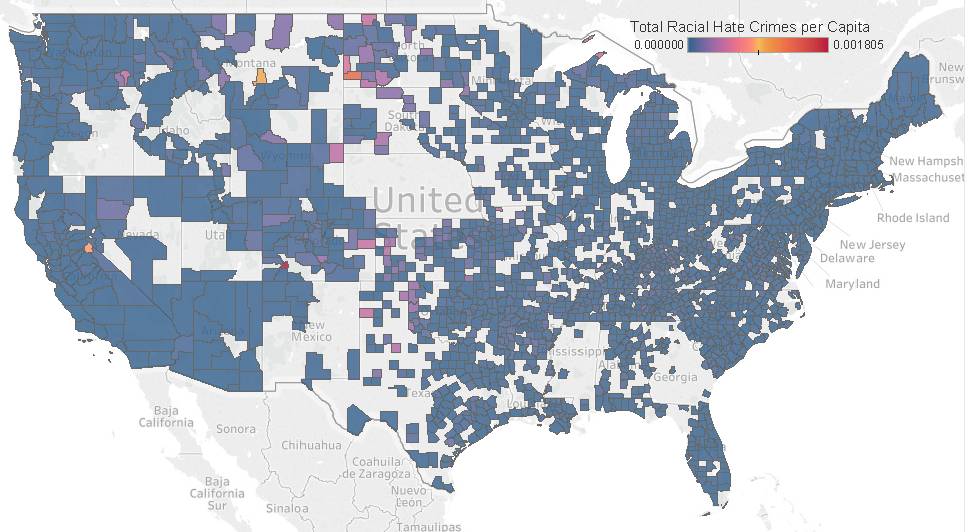
\includegraphics[scale = .6]{all_hc_percap_2005_2016.png}
        \caption{US Mainland Hate Crime Distribution per Capita 2005-2016}
        \label{fig:hc_cap_map}
    \end{figure}
    
\section{Empirical Strategy}

    This paper uses a difference-in-differences design to test whether people reporting a particular ancestry or national origin (such as Mexican or Nigerian) are less likely to report the commonly-corresponding racial or ethnic identity (such as Hispanic or Black, respectively) following an increase in racial crime in their county. This approach follows findings that show that ancestry and origin reporting is likely to be more stable than racial and ethnic identities \cite{antman15}. This paper measures whether the presence of hate crimes within a specific geographic area affect the reported identities of targeted groups within the same geography. 

		\begin{align*}
        \mathrm{GroupIdentity}_{ijt} =
        \alpha 
        &+ \beta_{0} \big( \mathrm{AntiGroupCrime}_{jt} \big)  \\
            &+ \beta_{1}  \big( \mathrm{AntiGroupCrime}_{jt} * \mathrm{GroupAncestryOnly}_{ijt} \big)  \\
            &+ \beta_{2}  \big( \mathrm{AntiGroupCrime}_{jt} * \mathrm{GroupAndOtherAncestry}_{ijt} \big)  \\
            &+ \mathrm{X}_{ijt} + \gamma_{t}  + \delta_{j} + \epsilon_{t} \\
                (Specification 1) 
        \end{align*}
        \begin{itemize}
            \item GroupIdentity: binary variable measuring whether individual identifies as the group targeted by a hate crime, within county j at time t 
            \item AntiGroupHateCrime: binary variable indicating the presence of any group-targeted hate crime, in a given county during a given year
            \item GroupAncestry: reported ancestry comprised of either fully or half of the group targeted by a hate crime, an individual at time t
        \end{itemize}

    As robustness checks, the specification was run on a variety of measurements of the presence of hate crimes including the sum and mean of hate crimes over the 11-year period in a given county, hate crimes measured relative to the counties' population and the county's population of targeted subpopulations, and type of hate crime. Furthermore, the specification was run with a lagged year for crimes that occur in year $x$, and racial \& ethnic affiliation in year $x+1$. Tables with results from additional robsustness checks are included in the appendix tables. 
    
    Individual fixed effects ($\mathrm{X}_{ijt}$) control for various demographic characteristics like the individuals' age, gender, education, and income. Other individual characteristics are binary variables measuring whether the individual is an immigrant, marriage status, and English proficiency. I also control for household characteristics like metropolitan status and home ownership. 
    
    County fixed effects ($\delta_{j}$) controls for overall county population and the percentage of the population that is composed of the targeted group. For instance, specifications with anti-Black crime and Black identity measure for the county's nominal Black population as well as the Black percentage of the county's population. 
    
    As an additional robustness check, specifications were also run using violent hate crimes, specifically. Violent hate crimes include those that either \say{involve force or threat of force} \cite{ucr}. Violent hate crimes are about 48,092 or 60\% of those reported in the Uniform Crime Report. Because of the particular terror that could be invoked by violent hate crimes, they could result in differential---perhaps stronger---outcomes. 
    
\section{Results}

    This paper uses various measures of the presence of hate crimes to understand on the effects of targeted racial hate crimes on the affected communities. Beginning with the binary measure of the presence of any targeted hate crime in a given county during a given year gives different results for Black and Hispanic identity. Table \ref{tab:any_anti_blk_yr} shows negative effects on Black identity in the presence of anti-Black hate crimes for individuals with exclusively Black ancestry and Black ancestry in combination with another ancestral association. There are apparently positive effects on Hispanic identity in the presence of anti-Hispanic hate crimes in a given area during a given year (Table \ref{tab:any_anti_hsp_yr}). 
    
    Lagged year hate crimes give similar results in terms of direction, but with a stronger magnitude for those with mixed ancestry and weaker magnitude for those with single ancestry (Appendix Tables \ref{tab:black_lag} \& \ref{tab:hisp_lag}). For violent hate crimes, the results for those with Black ancestry are consistently negative. For those with exclusively Black ancestry the results are slightly weaker and for those with Black and other ancestry the results are more strongly negative (Appendix Table \ref{tab:vio_any_anti_blk_yr}). For those with Hispanic ancestry, the results for violent hate crimes are similar in direction and magnitude (Appendix Table \ref{tab:vio_any_anti_hsp_yr}).  

        % Any Anti-Black in the Same Year & Black ID
        \begin{table}[!htbp] \centering
          \caption{Presence of Any Anti-Black Hate Crime \& Black Identity}
          \begin{tabular}{@{\extracolsep{5pt}}lc} 
            \\[-1.8ex]\hline 
            \hline \\[-1.8ex] 
             & \multicolumn{1}{c}{\small{Black Identification}} \\ 
            \hline \\[-1.8ex] 
             Anti-Black Crime & $-$0.003$^{***}$ \\
              & \small{(0.0001)} \\     
             Anti-Black Crime $\times$ Black Ancestry Only & $-$0.011$^{***}$ \\ 
              & \small{(0.0001)} \\ 
             Anti-Black Crime $\times$ Black Ancestry \& Other & $-$0.001$^{***}$ \\ 
              & \small{(0.001)} \\           
             Black Ancestry Only & 0.934$^{***}$ \\ 
              & \small{(0.001)} \\ 
             Black Ancestry \& Other & 0.913$^{***}$ \\ 
              & \small{(0.0002)} \\ 
            \hline \\[-1.8ex] 
            Observations & 15,024,310 \\ 
            R$^{2}$ & 0.883 \\ 
            Residual Std. Error & 1.237 (df = 15024291) \\ 
        \end{tabular} 
        \label{tab:any_anti_blk_yr}
        \end{table} 
        
        % Any Anti-Black in the Same Year & Black ID
        \begin{table}[!htbp] \centering 
          \caption{Presence of Any Anti-Hispanic Hate Crime \& Hispanic Identity} 
        \begin{tabular}{@{\extracolsep{5pt}}lc} 
        \\[-1.8ex]\hline 
        \hline \\[-1.8ex] 
         & \small{Hispanic Identification} \\ 
        \hline \\[-1.8ex] 
         Anti-Hispanic Crime & -0.003$^{***}$ \\ 
          & \small{(0.0001)} \\   
         Anti-Hispanic Crime $\times$ Hispanic Ancestry Only & 0.013$^{***}$ \\ 
          & \small{(0.001)} \\ 
         Anti-Hispanic Crime $\times$ Hispanic Ancestry \& Other & 0.018$^{***}$ \\ 
          & \small{(0.0002)} \\           
         Hispanic Ancestry Only & 0.942$^{***}$ \\ 
          & \small{(0.001)} \\ 
         Hispanic Ancestry  \& Other & 0.918$^{***}$ \\ 
          & \small{(0.0001)} \\ 
        \hline \\[-1.8ex] 
        Observations & 15,024,310 \\ 
        R$^{2}$ & 0.917 \\ 
        \small{Residual Std. Error & 0.115 (df = 12492405)} \\ 
        \end{tabular} 
        \label{tab:any_anti_hsp_yr}
        \end{table} 
    
    Another way to understand the effects of these crimes is through the lens of population size. Tables \ref{tab:anti_blk1000_yr} and \ref{tab:anti_hsp1000_yr} show the results of measuring targeted hate crimes per 1000 in a county. Results are consistent in terms of direction with the presence of any hate crime in a county over the given time period. These results are stronger for the presence of solely violent hate crimes (Appendix Tables \ref{tab:vio_anti_blk1000_yr} and \ref{tab:vio_anti_hsp1000_yr}). Those with any Black ancestry are less likely to identify as Black in the presence of violent hate crimes per 1000 and those with Hispanic ancestry are more likely to identify as Hispanic in the presence of violent hate crimes per 1000. This can speak to network effects that are more relevant within smaller communities. 
    
        % Anti-Black per 1000 in the Same Year & Black ID
        \begin{table}[!htbp] \centering
          \caption{Anti-Black Hate Crimes per 1000 \& Black Identity}
          \begin{tabular}{@{\extracolsep{5pt}}lc} 
            \\[-1.8ex]\hline 
            \hline \\[-1.8ex] 
             & \multicolumn{1}{c}{\small{Black Identification}} \\ 
            \hline \\[-1.8ex] 
             Anti-Black Crime per 1000 & 0.001 \\
              & \small{(0.001)} \\     
             Anti-Black Crime per 1000 $\times$ Black Ancestry Only & $-$0.079$^{***}$ \\ 
              & \small{(0.009)} \\ 
             Anti-Black Crime per 1000 $\times$ Black Ancestry \& Other & $-$0.144$^{***}$ \\ 
              & \small{(0.001)} \\           
             Black Ancestry Only & 0.932$^{***}$ \\ 
              & \small{(0.001)} \\ 
             Black Ancestry \& Other & 0.921$^{***}$ \\ 
              & \small{(0.0001)} \\ 
            \hline \\[-1.8ex] 
            Observations & 15,024,310 \\ 
            R$^{2}$ & 0.883 \\ 
            Residual Std. Error & 1.237 (df = 15024291) \\ 
        \end{tabular} 
        \label{tab:anti_blk1000_yr}
        \end{table} 
        
        % Anti-Hispanic per 1000 in the Same Year & Black ID
        \begin{table}[!htbp] \centering 
          \caption{Anti-Hispanic Hate Crimes per 1000 \& Hispanic Identity} 
        \begin{tabular}{@{\extracolsep{5pt}}lc} 
        \\[-1.8ex]\hline 
        \hline \\[-1.8ex] 
         & \small{Hispanic Identification} \\ 
        \hline \\[-1.8ex] 
         Anti-Hispanic Crime per 1000 & -0.044$^{***}$ \\ 
          & \small{(0.002)} \\   
         Anti-Hispanic Crime per 1000 $\times$ Hispanic Ancestry Only & 0.229$^{***}$ \\ 
          & \small{(0.021)} \\ 
         Anti-Hispanic Crime per 1000 $\times$ Hispanic Ancestry \& Other & 0.202$^{***}$ \\ 
          & \small{(0.004)} \\           
         Hispanic Ancestry Only & 0.945$^{***}$ \\ 
          & \small{(0.001)} \\ 
         Hispanic Ancestry  \& Other & 0.925$^{***}$ \\ 
          & \small{(0.0001)} \\ 
        \hline \\[-1.8ex] 
        Observations & 15,024,310 \\ 
        R$^{2}$ & 0.909 \\ 
        \small{Residual Std. Error & 0.115 (df = 12492405)} \\ 
        \end{tabular} 
        \label{tab:anti_hsp1000_yr}
        \end{table} 

    I also measured effects related to targeted hate crime per capita of a targeted group in a given county. To understand the strength of the effects on the targeted communities, I use a measure of hate crimes per capita of the affected group; for instance, anti-Hispanic hate crimes per Hispanic capita in a given county. This measure shows negative effects for both Black and Hispanic groups. Individuals with exclusively Black, Black and other, and Hispanic and other ancestry are less likely to align with Black, Black, and Hispanic identities, respectively. Table \ref{tab:any_anti_blkcap_yr} shows the results for Black identity and table \ref{tab:any_anti_hspcap_yr} shows the results for Hispanic identity. The effects of violent hate crimes are even stronger and more negative for those with mixed Black and mixed Hispanic ancestry (Appendix Tables \ref{tab:vio_any_anti_blkcap_yr} and \ref{tab:vio_any_anti_hspcap_yr}). Similar to the results with all hate crimes, the results for those with Hispanic and other ancestry are strongly negative. For those with exclusively Hispanic ancestry, the results remain positive and are also stronger. 
    
    This measure is an attempt to understand the effects of a targeted hate crime on a local community by understanding identity as it relates to the size of the specific community. Although the nominal amount of hate crimes may seem inconsequential, relative to the size of a community their impacts may be powerful. This relates back to the idea that hate crimes per capita tends to be higher in smaller communities, but measures with an understanding of the actual size of the targeted subpopulation.  
    
        % Anti-Black Hate Crimes per Black Capita
        \begin{table}[!htbp] \centering
          \caption{Anti-Black Hate Crimes per Black Capita \& Black Identity} 
          \begin{tabular}{@{\extracolsep{5pt}}lc} 
            \\[-1.8ex]\hline 
            \hline \\[-1.8ex] 
             & \multicolumn{1}{c}{\small{Black Identification}} \\ 
            \hline \\[-1.8ex] 
             Anti-Black Crime & 3.250$^{***}$ \\
             per Black Capita & \small{(0.099)} \\     
             Anti-Black Crime per Black Capita & $-$64.541$^{***}$ \\ 
             $\times$ Black Ancestry Only & \small{(0.0001)} \\ 
             Anti-Black Crime per Black Capita   & $-$163.524$^{***}$ \\ 
             $\times$ Black Ancestry \& Other & \small{(0.001)} \\           
             Black Ancestry Only & 0.931$^{***}$ \\ 
              & \small{(0.001)} \\ 
             Black Ancestry \& Other & 0.920$^{***}$ \\ 
              & \small{(0.0001)} \\ 
            \hline \\[-1.8ex] 
            Observations & 15,024,310 \\ 
            R$^{2}$ & 0.883 \\ 
            Residual Std. Error & 1.237 (df = 15024291) \\ 
        \end{tabular} 
        \label{tab:any_anti_blkcap_yr}
        \end{table} 
        
        % Anti-Hispanic Hate Crimes per Hispanic Capita
        \begin{table}[!htbp] \centering 
          \caption{Anti-Hispanic Hate Crimes per Hispanic Capita \& Hispanic Identity} 
        \begin{tabular}{@{\extracolsep{5pt}}lc} 
        \\[-1.8ex]\hline 
        \hline \\[-1.8ex] 
         & \small{Hispanic Identification} \\ 
        \hline \\[-1.8ex] 
         Anti-Hispanic Crime  & 6.199$^{***}$ \\ 
         per Hispanic Capita & \small{(0.466)} \\   
         Anti-Hispanic Crime per Hispanic Capita & 19.936\\ 
         $\times$  Hispanic Ancestry Only & \small{(13.396)} \\ 
         Anti-Hispanic Crime per Hispanic Capita   & $-$157.344$^{***}$ \\ 
         $\times$  Hispanic Ancestry \& Other & \small{(2.117)} \\           
         Hispanic Ancestry Only & 0.950$^{***}$ \\ 
          & \small{(0.0004)} \\ 
         Hispanic Ancestry  \& Other & 0.931$^{***}$ \\ 
          & \small{(0.0001)} \\ 
        \hline \\[-1.8ex] 
        Observations & 15,024,310 \\ 
        R$^{2}$ & 0.909 \\ 
        \small{Residual Std. Error & 1.297 (df = 15024291)} \\ 
        \end{tabular} 
        \label{tab:any_anti_hspcap_yr}
        \end{table} 

    While both Black and Hispanic identity was related to targeted hate crimes in a given geography, the results for Black respondents were more robust and consistently negative. This finding may be somewhat unexpected given previous findings on ethnic attrition related to Hispanic identity. That said, there are several contributing factors to this difference. The first is the difference in the proportion of anti-Black hate crimes and the proportion of anti-Hispanic hate crimes relative to both groups' proportions of the population. While Black people are 13 percent of the population, anti-Black hate crimes are 33 percent of all hate crimes and 54 percent of all racially-motivated hate crimes. Eighteen percent of the population identifies as Hispanic or Latino, and anti-Hispanic hate crimes constitute seven percent of all hate crimes and 11 percent of all racially-motivated hate crimes. That said, there are almost certainly under-reporting issues within both groups. Crime under-reporting has been associated with police distrust in relation to race and immigration status, topics pertinent to both communities. 

\newpage

\section*{Appendices}
\appendix

\section{Robustness Checks}
\subsection{Sum of Hate Crimes}
    \begin{table}[!htbp] \centering 
      \caption{} 
      \label{} 
    \begin{tabular}{@{\extracolsep{5pt}}lc} 
    \\[-1.8ex]\hline 
    \hline \\[-1.8ex] 
     & \multicolumn{1}{c}{\textit{Dependent variable:}} \\ 
    \cline{2-2} 
    \\[-1.8ex] & black \\ 
     & Black Identification \\ 
    \hline \\[-1.8ex] 
     Black Ancestry Only & 0.931$^{***}$ \\ 
      & (0.001) \\ 
     Sum Anti-Black Hate Crimes & $-$0.0001$^{***}$ \\ 
      & (0.00000) \\ 
     Black Ancestry \& Other & 0.914$^{***}$ \\ 
      & (0.0001) \\ 
     Black Ancestry Only $\times$ Sum Anti-Black Hate Crimes & $-$0.001$^{***}$ \\ 
      & (0.0001) \\ 
     Sum Anti-Black Hate Crimes:Black Ancestry \& Other & $-$0.0003$^{***}$ \\ 
      & (0.00001) \\ 
    \hline \\[-1.8ex] 
    Observations & 15,024,310 \\ 
    R$^{2}$ & 0.883 \\ 
    Adjusted R$^{2}$ & 0.883 \\ 
    Residual Std. Error & 1.237 (df = 15024291) \\ 
    \hline 
    \hline \\[-1.8ex] 
    \textit{Note:}  & \multicolumn{1}{r}{$^{*}$p$<$0.1; $^{**}$p$<$0.05; $^{***}$p$<$0.01} \\ 
    \end{tabular} 
    \end{table} 

    \begin{table}[!htbp] \centering 
      \caption{} 
      \label{} 
    \begin{tabular}{@{\extracolsep{5pt}}lc} 
    \\[-1.8ex]\hline 
    \hline \\[-1.8ex] 
     & \multicolumn{1}{c}{\textit{Dependent variable:}} \\ 
    \cline{2-2} 
    \\[-1.8ex] & hisp \\ 
     & hisp Identification \\ 
    \hline \\[-1.8ex] 
     Hispanic Ancestry Only & 0.946$^{***}$ \\ 
      & (0.0005) \\ 
     Anti Hispanic Crime Sum  & $-$0.0005$^{***}$ \\ 
      & (0.00001) \\ 
     Hispanic Ancestry \& Other & 0.923$^{***}$ \\ 
      & (0.0001) \\ 
     Hispanic Ancestry Only $\times$Anti Hispanic Crime Sum  & 0.001$^{***}$ \\ 
      & (0.00005) \\ 
     Anti Hispanic Crime Sum $\times$ Hispanic Ancestry \& Other & 0.001$^{***}$ \\ 
      & (0.00001) \\ 
    \hline \\[-1.8ex] 
    Observations & 15,024,310 \\ 
    R$^{2}$ & 0.909 \\ 
    Adjusted R$^{2}$ & 0.909 \\ 
    Residual Std. Error & 1.297 (df = 15024291) \\ 
    \hline 
    \hline \\[-1.8ex] 
    \textit{Note:}  & \multicolumn{1}{r}{$^{*}$p$<$0.1; $^{**}$p$<$0.05; $^{***}$p$<$0.01} \\ 
    \end{tabular} 
    \end{table} 

\newpage
\subsection{Mean of Hate Crimes}
    \begin{table}[!htbp] \centering 
      \caption{} 
      \label{} 
    \begin{tabular}{@{\extracolsep{5pt}}lc} 
    \\[-1.8ex]\hline 
    \hline \\[-1.8ex] 
     & \multicolumn{1}{c}{\textit{Dependent variable:}} \\ 
    \cline{2-2} 
    \\[-1.8ex] & black \\ 
     & Black Identification \\ 
    \hline \\[-1.8ex] 
     Black Ancestry Only & 0.931$^{***}$ \\ 
      & (0.001) \\ 
     Anti Black Crime Mean  & $-$0.002$^{***}$ \\ 
      & (0.00004) \\ 
     Black Ancestry \& Other & 0.914$^{***}$ \\ 
      & (0.0001) \\ 
     Black Ancestry Only $\times$ Anti Black Crime Mean  & $-$0.008$^{***}$ \\ 
      & (0.001) \\ 
     Anti Black Crime Mean $\times$  Black Ancestry \& Other & $-$0.003$^{***}$ \\ 
      & (0.0001) \\ 
    \hline \\[-1.8ex] 
    Observations & 15,024,310 \\ 
    R$^{2}$ & 0.883 \\ 
    Adjusted R$^{2}$ & 0.883 \\ 
    Residual Std. Error & 1.237 (df = 15024291) \\ 
    \hline 
    \hline \\[-1.8ex] 
    \textit{Note:}  & \multicolumn{1}{r}{$^{*}$p$<$0.1; $^{**}$p$<$0.05; $^{***}$p$<$0.01} \\ 
    \end{tabular} 
    \end{table} 

    \begin{table}[!htbp] \centering 
      \caption{} 
      \label{} 
    \begin{tabular}{@{\extracolsep{5pt}}lc} 
    \\[-1.8ex]\hline 
    \hline \\[-1.8ex] 
     & \multicolumn{1}{c}{\textit{Dependent variable:}} \\ 
    \cline{2-2} 
    \\[-1.8ex] & hisp \\ 
     & hisp Identification \\ 
    \hline \\[-1.8ex] 
     Hispanic Ancestry Only & 0.945$^{***}$ \\ 
      & (0.0005) \\ 
     Anti Black Crime Mean  & $-$0.0004$^{***}$ \\ 
      & (0.00001) \\ 
     Hispanic Ancestry Only $\times$Anti Black Crime Mean  & 0.001$^{***}$ \\ 
      & (0.00005) \\ 
     Anti Hispanic Crime Mean $\times$ Hispanic Ancestry \& Other & 0.002$^{***}$ \\ 
      & (0.00001) \\ 
    \hline \\[-1.8ex] 
    Observations & 15,024,310 \\ 
    R$^{2}$ & 0.909 \\ 
    Adjusted R$^{2}$ & 0.909 \\ 
    Residual Std. Error & 1.296 (df = 15024291) \\ 
    \hline 
    \hline \\[-1.8ex] 
    \textit{Note:}  & \multicolumn{1}{r}{$^{*}$p$<$0.1; $^{**}$p$<$0.05; $^{***}$p$<$0.01} \\ 
    \end{tabular} 
    \end{table} 


\newpage
\subsection{Total Hate Crimes in a County 2005-2016}
    \begin{table}[!htbp] \centering 
      \caption{} 
      \label{} 
    \begin{tabular}{@{\extracolsep{5pt}}lc} 
    \\[-1.8ex]\hline 
    \hline \\[-1.8ex] 
     & \multicolumn{1}{c}{\textit{Dependent variable:}} \\ 
    \cline{2-2} 
    \\[-1.8ex] & black \\ 
     & Black Identification \\ 
    \hline \\[-1.8ex] 
     Black Ancestry Only & 0.930$^{***}$ \\ 
      & (0.001) \\ 
     Anti-Black Total & $-$0.00001$^{***}$ \\ 
      & (0.00000) \\ 
     Black Ancestry \& Other & 0.915$^{***}$ \\ 
      & (0.0001) \\ 
     Black Ancestry Only $\times$ Anti-Black Total & $-$0.00005$^{***}$ \\ 
      & (0.00001) \\ 
     Anti-Black Total $\times$ Black Ancestry \& Other & $-$0.00003$^{***}$ \\ 
      & (0.00000) \\ 
    \hline \\[-1.8ex] 
    Observations & 15,024,310 \\ 
    R$^{2}$ & 0.883 \\ 
    Adjusted R$^{2}$ & 0.883 \\ 
    Residual Std. Error & 1.237 (df = 15024291) \\ 
    \hline 
    \hline \\[-1.8ex] 
    \textit{Note:}  & \multicolumn{1}{r}{$^{*}$p$<$0.1; $^{**}$p$<$0.05; $^{***}$p$<$0.01} \\ 
    \end{tabular} 
    \end{table} 




\newpage    
\subsection{Targeted Crime per 1000 of Targeted Population}
    \begin{table}[!htbp] \centering 
      \caption{} 
      \label{} 
    \begin{tabular}{@{\extracolsep{5pt}}lc} 
    \\[-1.8ex]\hline 
    \hline \\[-1.8ex] 
     & \multicolumn{1}{c}{\textit{Dependent variable:}} \\ 
    \cline{2-2} 
    \\[-1.8ex] & black \\ 
     & Black Identification \\ 
    \hline \\[-1.8ex] 
     Black Ancestry Only & 0.934$^{***}$ \\ 
      & (0.001) \\ 
     Black Crime per Black 1000 & 0.0005$^{***}$ \\ 
      & (0.00001) \\ 
     Black Ancestry \& Other & 0.926$^{***}$ \\ 
      & (0.0001) \\ 
     Black Ancestry Only $\times$ Black Crime per Black 1000 & $-$0.010$^{***}$ \\ 
      & (0.001) \\ 
     Black Crime per Black 1000 $\times$Black Ancestry \& Other & $-$0.023$^{***}$ \\ 
      & (0.0001) \\ 
    \hline \\[-1.8ex] 
    Observations & 15,024,310 \\ 
    R$^{2}$ & 0.884 \\ 
    Adjusted R$^{2}$ & 0.884 \\ 
    Residual Std. Error & 1.233 (df = 15024291) \\ 
    \hline 
    \hline \\[-1.8ex] 
    \textit{Note:}  & \multicolumn{1}{r}{$^{*}$p$<$0.1; $^{**}$p$<$0.05; $^{***}$p$<$0.01} \\ 
    \end{tabular} 
    \end{table} 

    \begin{table}[!htbp] \centering 
      \caption{} 
      \label{} 
    \begin{tabular}{@{\extracolsep{5pt}}lc} 
    \\[-1.8ex]\hline 
    \hline \\[-1.8ex] 
     & \multicolumn{1}{c}{\textit{Dependent variable:}} \\ 
    \cline{2-2} 
    \\[-1.8ex] & hisp \\ 
     & hisp Identification \\ 
    \hline \\[-1.8ex] 
     Hispanic Ancestry Only & 0.945$^{***}$ \\ 
      & (0.001) \\ 
     Anti-Hispanic Crimes per 1000 & $-$0.044$^{***}$ \\ 
      & (0.002) \\ 
     Hispanic Ancestry \& Other & 0.925$^{***}$ \\ 
      & (0.0001) \\ 
     Hispanic Ancestry Only $\times$ Anti-Hispanic Crimes per 1000 & 0.229$^{***}$ \\ 
      & (0.021) \\ 
     Anti-Hispanic Crimes per 1000 $\times$ Hispanic Ancestry \& Other & 0.202$^{***}$ \\ 
      & (0.004) \\ 
    \hline \\[-1.8ex] 
    Observations & 15,024,310 \\ 
    R$^{2}$ & 0.909 \\ 
    Adjusted R$^{2}$ & 0.909 \\ 
    Residual Std. Error & 1.297 (df = 15024291) \\ 
    \hline 
    \hline \\[-1.8ex] 
    \textit{Note:}  & \multicolumn{1}{r}{$^{*}$p$<$0.1; $^{**}$p$<$0.05; $^{***}$p$<$0.01} \\ 
    \end{tabular} 
    \end{table} 


\newpage
\section{Results with Violent Hate Crimes}
    As a robustness check, I also ran regressions with only violent hate crimes. These results reinforce the original results with all hate crimes. Violent hate crimes reinforced the effects of all hate crimes, and in most cases were stronger. 

    \subsection{Any Violent Hate Crimes}

        % Any Anti-Black in the Same Year & Black ID
        \begin{table}[!htbp] \centering
          \caption{Presence of Any Anti-Black Hate Crime \& Black Identity}
          \begin{tabular}{@{\extracolsep{5pt}}lc} 
            \\[-1.8ex]\hline 
            \hline \\[-1.8ex] 
             & \multicolumn{1}{c}{\small{Black Identification}} \\ 
            \hline \\[-1.8ex] 
             Anti-Black Crime & $-$0.002$^{***}$ \\
              & \small{(0.0001)} \\     
             Anti-Black Crime $\times$ Black Ancestry Only & $-$0.005$^{***}$ \\ 
              & \small{(0.002)} \\ 
             Anti-Black Crime $\times$ Black Ancestry \& Other & 0.005$^{***}$ \\ 
              & \small{(0.0003)} \\           
             Black Ancestry Only & 0.929$^{***}$ \\ 
              & \small{(0.002)} \\ 
             Black Ancestry \& Other & 0.908$^{***}$ \\ 
              & \small{(0.0002)} \\ 
            \hline \\[-1.8ex] 
            Observations & 15,024,310 \\ 
            R$^{2}$ & 0.885 \\ 
        \end{tabular} 
        \label{tab:vio_any_anti_blk_yr}
        \end{table} 
        
        % Any Anti-Black in the Same Year & Black ID
        \begin{table}[!htbp] \centering 
          \caption{Presence of Any Anti-Hispanic Hate Crime \& Hispanic Identity} 
        \begin{tabular}{@{\extracolsep{5pt}}lc} 
        \\[-1.8ex]\hline 
        \hline \\[-1.8ex] 
         & \small{Hispanic Identification} \\ 
        \hline \\[-1.8ex] 
         Anti-Hispanic Crime & -0.004$^{***}$ \\ 
          & \small{(0.0001)} \\   
         Anti-Hispanic Crime $\times$ Hispanic Ancestry Only & 0.018$^{***}$ \\ 
          & \small{(0.001)} \\ 
         Anti-Hispanic Crime $\times$ Hispanic Ancestry \& Other & 0.019$^{***}$ \\ 
          & \small{(0.0002)} \\           
         Hispanic Ancestry Only & 0.938$^{***}$ \\ 
          & \small{(0.001)} \\ 
         Hispanic Ancestry  \& Other & 0.917$^{***}$ \\ 
          & \small{(0.0002)} \\ 
        \hline \\[-1.8ex] 
        Observations & 15,024,310 \\ 
        R$^{2}$ & 0.917 \\ 
        \end{tabular} 
        \label{tab:vio_any_anti_hsp_yr}
        \end{table} 
\newpage

    \subsection{Violent Crime per 1000}

        % Anti-Black per 1000 in the Same Year & Black ID
        \begin{table}[!htbp] \centering
          \caption{Anti-Black Hate Crimes per 1000 \& Black Identity}
          \begin{tabular}{@{\extracolsep{5pt}}lc} 
            \\[-1.8ex]\hline 
            \hline \\[-1.8ex] 
             & \multicolumn{1}{c}{\small{Black Identification}} \\ 
            \hline \\[-1.8ex] 
             Anti-Black Crime per 1000 & 0.008 \\
              & \small{(0.007)} \\     
             Anti-Black Crime per 1000 $\times$ Black Ancestry Only & $-$1.078$^{***}$ \\ 
              & \small{(0.135)} \\ 
             Anti-Black Crime per 1000 $\times$ Black Ancestry \& Other & $-$1.268$^{***}$ \\ 
              & \small{(0.018)} \\           
             Black Ancestry Only & 0.931$^{***}$ \\ 
              & \small{(0.001)} \\ 
             Black Ancestry \& Other & 0.917$^{***}$ \\ 
              & \small{(0.0001)} \\ 
            \hline \\[-1.8ex] 
            Observations & 15,024,310 \\ 
            R$^{2}$ & 0.884 \\ 
            Residual Std. Error & 1.235 (df = 15024291) \\ 
        \end{tabular} 
        \label{tab:vio_anti_blk1000_yr}
        \end{table} 
        
        % Anti-Hispanic per 1000 in the Same Year & Black ID
        \begin{table}[!htbp] \centering 
          \caption{Anti-Hispanic Hate Crimes per 1000 \& Hispanic Identity} 
        \begin{tabular}{@{\extracolsep{5pt}}lc} 
        \\[-1.8ex]\hline 
        \hline \\[-1.8ex] 
         & \small{Hispanic Identification} \\ 
        \hline \\[-1.8ex] 
         Anti-Hispanic Crime per 1000 & -0.221$^{***}$ \\ 
          & \small{(0.018)} \\   
         Anti-Hispanic Crime per 1000 $\times$ Hispanic Ancestry Only & 1.900$^{***}$ \\ 
          & \small{(0.230)} \\ 
         Anti-Hispanic Crime per 1000 $\times$ Hispanic Ancestry \& Other & 0.994$^{***}$ \\ 
          & \small{(0.040)} \\           
         Hispanic Ancestry Only & 0.947$^{***}$ \\ 
          & \small{(0.0005)} \\ 
         Hispanic Ancestry  \& Other & 0.927$^{***}$ \\ 
          & \small{(0.0001)} \\ 
        \hline \\[-1.8ex] 
        Observations & 15,024,310 \\ 
        R$^{2}$ & 0.909 \\ 
        \small{Residual Std. Error & 1.297 (df = 12492405)} \\ 
        \end{tabular} 
        \label{tab:vio_anti_hsp1000_yr}
        \end{table} 
\newpage

    \subsection{Violent Hate Crimes per Targeted Population Capita}

        % Anti-Black Hate Crimes per Black Capita
        \begin{table}[!htbp] \centering
          \caption{Anti-Black Hate Crimes per Black Capita \& Black Identity} 
          \begin{tabular}{@{\extracolsep{5pt}}lc} 
            \\[-1.8ex]\hline 
            \hline \\[-1.8ex] 
             & \multicolumn{1}{c}{\small{Black Identification}} \\ 
            \hline \\[-1.8ex] 
             Anti-Black Crime & 4.262$^{***}$ \\
             per Black Capita & \small{(0.133)} \\     
             Anti-Black Crime per Black Capita & $-$66.377$^{***}$ \\ 
             $\times$ Black Ancestry Only & \small{(6.871)} \\ 
             Anti-Black Crime per Black Capita   & $-$214.966$^{***}$ \\ 
             $\times$ Black Ancestry \& Other & \small{(0.952)} \\           
             Black Ancestry Only & 0.930$^{***}$ \\ 
              & \small{(0.001)} \\ 
             Black Ancestry \& Other & 0.919$^{***}$ \\ 
              & \small{(0.0001)} \\ 
            \hline \\[-1.8ex] 
            Observations & 15,024,310 \\ 
            R$^{2}$ & 0.884 \\ 
            Residual Std. Error & 1.235 (df = 15024291) \\ 
        \end{tabular} 
        \label{tab:vio_any_anti_blkcap_yr}
        \end{table} 
        
        % Anti-Hispanic Hate Crimes per Hispanic Capita
        \begin{table}[!htbp] \centering 
          \caption{Anti-Hispanic Hate Crimes per Hispanic Capita \& Hispanic Identity} 
        \begin{tabular}{@{\extracolsep{5pt}}lc} 
        \\[-1.8ex]\hline 
        \hline \\[-1.8ex] 
         & \small{Hispanic Identification} \\ 
        \hline \\[-1.8ex] 
         Anti-Hispanic Crime  & 7.028$^{***}$ \\ 
         per Hispanic Capita & \small{(0.582)} \\   
         Anti-Hispanic Crime per Hispanic Capita & 38.801\\ 
         $\times$  Hispanic Ancestry Only & \small{(16.669)} \\
         Anti-Hispanic Crime per Hispanic Capita   & $-$184.153$^{***}$ \\ 
         $\times$  Hispanic Ancestry \& Other & \small{(2.748)} \\           
         Hispanic Ancestry Only & 0.950$^{***}$ \\ 
          & \small{(0.0004)} \\ 
         Hispanic Ancestry  \& Other & 0.930$^{***}$ \\ 
          & \small{(0.0001)} \\ 
        \hline \\[-1.8ex] 
        Observations & 15,024,310 \\ 
        R$^{2}$ & 0.909 \\ 
        \small{Residual Std. Error & 1.297 (df = 15024291)} \\ 
        \end{tabular} 
        \label{tab:vio_any_anti_hspcap_yr}
        \end{table} 
        
\newpage
\section{Results with Lagged Year}
\subsection{Any Targeted Hate Crime}
    \begin{table}[!htbp] \centering 
      \caption{} 
      \label{} 
    \begin{tabular}{@{\extracolsep{5pt}}lc} 
    \\[-1.8ex]\hline 
    \hline \\[-1.8ex] 
     & \multicolumn{1}{c}{\textit{Dependent variable:}} \\ 
    \cline{2-2} 
    \\[-1.8ex] & black \\ 
     & Black Identification \\ 
    \hline \\[-1.8ex] 
     Black Ancestry Only & 0.932$^{***}$ \\ 
      & (0.001) \\ 
     Any Anti-Black Crime  & $-$0.002$^{***}$ \\ 
      & (0.0001) \\ 
     Black Ancestry \& Other & 0.916$^{***}$ \\ 
      & (0.0002) \\ 
     Black Ancestry Only $\times$ Any Anti-Black Crime  & $-$0.009$^{***}$ \\ 
      & (0.001) \\ 
     Any Anti-Black Crime $\times$ Black Ancestry \& Other & $-$0.006$^{***}$ \\ 
      & (0.0002) \\ 
    \hline \\[-1.8ex] 
    Observations & 15,024,310 \\ 
    R$^{2}$ & 0.883 \\ 
    Adjusted R$^{2}$ & 0.883 \\ 
    Residual Std. Error & 1.237 (df = 15024291) \\ 
    \hline 
    \hline \\[-1.8ex] 
    \textit{Note:}  & \multicolumn{1}{r}{$^{*}$p$<$0.1; $^{**}$p$<$0.05; $^{***}$p$<$0.01} \\ 
    \label{tab:black_lag}
    \end{tabular} 
    \end{table} 

    \begin{table}[!htbp] \centering 
      \caption{} 
      \label{} 
    \begin{tabular}{@{\extracolsep{5pt}}lc} 
    \\[-1.8ex]\hline 
    \hline \\[-1.8ex] 
     & \multicolumn{1}{c}{\textit{Dependent variable:}} \\ 
    \cline{2-2} 
    \\[-1.8ex] & hisp \\ 
     & hisp Identification \\ 
    \hline \\[-1.8ex] 
     Hispanic Ancestry Only & 0.943$^{***}$ \\ 
      & (0.001) \\ 
     Any Anti-Hispanic Crime  & $-$0.003$^{***}$ \\ 
      & (0.0001) \\ 
     Hispanic Ancestry Only $\times$ Any Anti-Hispanic Crime  & 0.012$^{***}$ \\ 
      & (0.001) \\ 
     Any Anti-Hispanic Crime $\times$ Hispanic Ancestry \& Other & 0.018$^{***}$ \\ 
      & (0.0002) \\ 
    \hline \\[-1.8ex] 
    Observations & 15,024,310 \\ 
    R$^{2}$ & 0.909 \\ 
    Adjusted R$^{2}$ & 0.909 \\ 
    Residual Std. Error & 1.297 (df = 15024291) \\ 
    F Statistic & 8,360,458.000$^{***}$ (df = 18; 15024291) \\ 
    \hline 
    \hline \\[-1.8ex] 
    \textit{Note:}  & \multicolumn{1}{r}{$^{*}$p$<$0.1; $^{**}$p$<$0.05; $^{***}$p$<$0.01} \\ 
    \end{tabular} 
    \label{tab:hisp_lag}
    \end{table} 

\newpage
\subsection{Crimes per 1000}
    \begin{table}[!htbp] \centering 
      \caption{} 
      \label{} 
    \begin{tabular}{@{\extracolsep{5pt}}lc} 
    \\[-1.8ex]\hline 
    \hline \\[-1.8ex] 
     & \multicolumn{1}{c}{\textit{Dependent variable:}} \\ 
    \cline{2-2} 
    \\[-1.8ex] & black \\ 
     & Black Identification \\ 
    \hline \\[-1.8ex] 
     Black Ancestry Only & 0.931$^{***}$ \\ 
      & (0.001) \\ 
     Anti-Black Crime per 1000 & 0.020$^{***}$ \\ 
      & (0.005) \\ 
     Black Ancestry Only $\times$ Anti-Black Crime per 1000 & $-$0.756$^{***}$ \\ 
      & (0.098) \\ 
     Anti-Black Crime per 1000 $\times$ Black Ancestry \& Other & $-$0.968$^{***}$ \\
      & (0.013) \\ 
    \hline \\[-1.8ex] 
    Observations & 15,024,310 \\ 
    R$^{2}$ & 0.883 \\ 
    Adjusted R$^{2}$ & 0.883 \\ 
    Residual Std. Error & 1.237 (df = 15024291) \\ 
    \hline 
    \hline \\[-1.8ex] 
    \textit{Note:}  & \multicolumn{1}{r}{$^{*}$p$<$0.1; $^{**}$p$<$0.05; $^{***}$p$<$0.01} \\ 
    \end{tabular} 
    \end{table} 
    
    \begin{table}[!htbp] \centering 
      \caption{} 
      \label{} 
    \begin{tabular}{@{\extracolsep{5pt}}lc} 
    \\[-1.8ex]\hline 
    \hline \\[-1.8ex] 
     & \multicolumn{1}{c}{\textit{Dependent variable:}} \\ 
    \cline{2-2} 
    \\[-1.8ex] & hisp \\ 
     & hisp Identification \\ 
    \hline \\[-1.8ex] 
     Hispanic Ancestry Only & 0.948$^{***}$ \\ 
      & (0.0005) \\ 
     Anti-Hispanic Crimes per 1000 & $-$0.188$^{***}$ \\ 
      & (0.014) \\ 
     Hispanic Ancestry Only $\times$ Anti-Hispanic Crimes per 1000 & 1.056$^{***}$ \\ 
      & (0.188) \\ 
     Anti-Hispanic Crimes per 1000 $\times$ Hispanic Ancestry \& Other & 0.882$^{***}$ \\ 
      & (0.034) \\ 
    \hline \\[-1.8ex] 
    Observations & 15,024,310 \\ 
    R$^{2}$ & 0.909 \\ 
    Adjusted R$^{2}$ & 0.909 \\ 
    Residual Std. Error & 1.297 (df = 15024291) \\ 
    \hline 
    \hline \\[-1.8ex] 
    \textit{Note:}  & \multicolumn{1}{r}{$^{*}$p$<$0.1; $^{**}$p$<$0.05; $^{***}$p$<$0.01} \\ 
    \end{tabular} 
    \end{table}     
    
\newpage    
\subsection{Crimes per targeted population}
    \begin{table}[!htbp] \centering 
      \caption{} 
      \label{} 
    \begin{tabular}{@{\extracolsep{5pt}}lc} 
    \\[-1.8ex]\hline 
    \hline \\[-1.8ex] 
     & \multicolumn{1}{c}{\textit{Dependent variable:}} \\ 
    \cline{2-2} 
    \\[-1.8ex] & black \\ 
     & Black Identification \\ 
    \hline \\[-1.8ex] 
     Black Ancestry Only & 0.931$^{***}$ \\ 
      & (0.001) \\ 
      Anti-Black Crime per Black Capita  & 3.455$^{***}$ \\ 
      & (0.101) \\ 
     Black Ancestry Only: Anti-Black Crime per Black Capita  & $-$56.606$^{***}$ \\ 
      & (4.882) \\ 
      Anti-Black Crime per Black Capita $\times$ Black Ancestry \& Other & $-$161.812$^{***}$ \\ 
      & (0.689) \\ 
    \hline \\[-1.8ex] 
    Observations & 15,024,310 \\ 
    R$^{2}$ & 0.884 \\ 
    Adjusted R$^{2}$ & 0.884 \\ 
    Residual Std. Error & 1.235 (df = 15024291) \\ 
    \hline 
    \hline \\[-1.8ex] 
    \textit{Note:}  & \multicolumn{1}{r}{$^{*}$p$<$0.1; $^{**}$p$<$0.05; $^{***}$p$<$0.01} \\ 
    \end{tabular} 
    \end{table} 
    
    \begin{table}[!htbp] \centering 
      \caption{} 
      \label{} 
    \begin{tabular}{@{\extracolsep{5pt}}lc} 
    \\[-1.8ex]\hline 
    \hline \\[-1.8ex] 
     & \multicolumn{1}{c}{\textit{Dependent variable:}} \\ 
    \cline{2-2} 
    \\[-1.8ex] & hisp \\ 
     & hisp Identification \\ 
    \hline \\[-1.8ex] 
     Hispanic Ancestry Only & 0.950$^{***}$ \\ 
      & (0.0004) \\ 
     Anti Hispanic Crime per Hispanic Capita  & 5.510$^{***}$ \\ 
      & (0.472) \\ 
     Hispanic Ancestry Only $\times$ Anti Hispanic Crime per Hispanic Capita  & 18.909 \\ 
      & (13.045) \\ 
     Anti Hispanic Crime per Hispanic Capita $\times$ Hispanic Ancestry \& Other & $-$121.678$^{***}$ \\ 
      & (2.085) \\ 
    \hline \\[-1.8ex] 
    Observations & 15,024,310 \\ 
    R$^{2}$ & 0.909 \\ 
    Adjusted R$^{2}$ & 0.909 \\ 
    Residual Std. Error & 1.297 (df = 15024291) \\ 
    \hline 
    \hline \\[-1.8ex] 
    \textit{Note:}  & \multicolumn{1}{r}{$^{*}$p$<$0.1; $^{**}$p$<$0.05; $^{***}$p$<$0.01} \\ 
    \end{tabular} 
    \end{table} 


\newpage
\begin{thebibliography}{9}
    \bibitem{antman15} 
    Antman, Francisca and Brian Duncan. 
    2015.
    "Incentive to Identify: Racial Identity in the Age of Affirmative Action". 
    \textit{Review of Economics and Statistics} 97 (3): 710–13. doi:http://www.mitpressjournals.org/loi/rest.

    \bibitem{antman16} 
    Antman, Francisca, Brian Duncan, and Stephen J. Trejo. 
    2016.
    "Ethnic Attrition and the Observed Health of Later-Generation Mexican Americans". 
    \textit{American Economic Review} 106 (5): 467–71. doi:http://www.aeaweb.org/aer/.

    \bibitem{ipums} 
    Ruggles, Steven, Sarah Flood, Ronald Goeken, Josiah Grover, Erin Meyer, Jose Pacas and Matthew Sobek. 2019. 
    IPUMS USA: Version 9.0 [dataset]. 
    IPUMS.
    doi: https://doi.org/10.18128/D010.V9.0
    
    \bibitem{ucr}
    United States Department of Justice Federal Bureau of Investigation. 
    Uniform Crime Reporting Program Data [United States]: Hate Crime Data, 2005-2016 [Record-Type Files]. 
    Inter-university Consortium for Political and Social Research [distributor].
    doi: https://doi.org/10.3886/ICPSR25107.v1.

\end{thebibliography}

\end{document}